\documentclass[12pt, oneside]{article}
\usepackage[letterpaper, margin=1in, headsep=0.5in]{geometry}
\usepackage[english]{babel}
\usepackage[utf8]{inputenc}
\usepackage{amsmath}
\usepackage{amsfonts}
\usepackage{amssymb}
\usepackage{tikz}
\usetikzlibrary{quotes, angles}
\usepackage{graphicx}
%\usepackage{pgfplots}
%\pgfplotsset{width=10cm,compat=1.9}
%\usepgfplotslibrary{statistics}
%\usepackage{pgfplotstable}
%\usepackage{tkz-fct}
%\usepackage{venndiagram}
\usepackage{multicol}

\usepackage{fancyhdr}
\pagestyle{fancy}
\fancyhf{}
\rhead{\thepage \\Name: \hspace{1.5in}.\\}
\lhead{BECA / Dr. Huson / 10.3 Geometry\\* 5 December 2018}

\renewcommand{\headrulewidth}{0pt}

\begin{document}
\subsection*{Do Now: Graphing systems}
Show your work. For graphs, use a pencil and straight edge.
  \begin{enumerate}

    \item Graph the two lines after filling in the values in the blanks.\\[0.5cm]
    Label both lines and the solution to the system, the intersection, as a coordinate pair.\\

    \begin{multicols}{2}
      $y=\frac{2}{3} x -5$ \\
      $y=-1 x +5$
    \end{multicols}
    \begin{multicols}{2}
      \raggedcolumns
      \begin{enumerate}
        \item $y$-intercept $= \rule{2cm}{0.15mm}$ \\[0.5cm]
        \item Slope \hspace{0.7cm} $= \rule{2cm}{0.15mm}$\\[0.5cm]
      \end{enumerate}
      \begin{enumerate}
        \item $y$-intercept $= \rule{2cm}{0.15mm}$ \\[0.5cm]
        \item Slope \hspace{0.7cm} $= \rule{2cm}{0.15mm}$\\[0.5cm]
      \end{enumerate}
    \end{multicols}

    \begin{center} %4 quadrant regents grid w T-Chart
    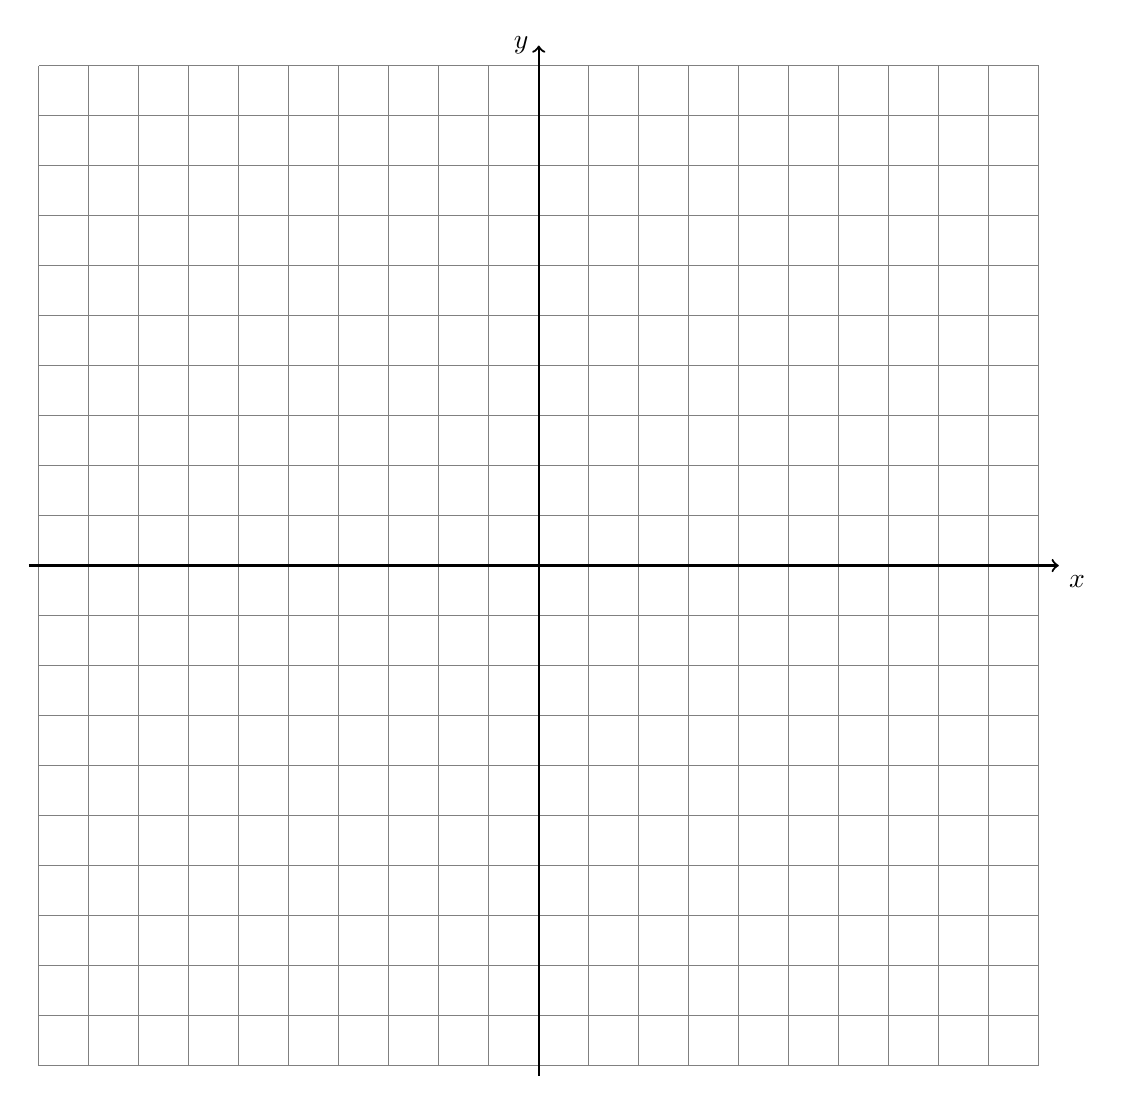
\begin{tikzpicture}[scale=.635]
      \draw [help lines] (-10,-10) grid (10,10);
      \draw [thick, ->] (-10.2,0) -- (10.4,0) node [below right] {$x$};
      \draw [thick, ->] (0,-10.2)--(0,10.4) node [left] {$y$};
    \end{tikzpicture}
    \end{center}




\end{enumerate}
\end{document}
